\section{SSL}
SSL är ett väldigt väl använt protokoll som man finner på nätet när en säker anslutning krävs. Med SSL förhindrar man tjuvlyssning på nätverket, vilket är en viktig faktor som gör protokollet säkert. 

Protokollet befinner sig mellan de två översta lagren i TCP/IP modellen, transportlagret och applikationslagret.
Eftersom protkollet används för säkra anslutningar på nätet faller det i sin natur att SSL används mestadels i Hypertext Transfer Protocol (HTTP) \cite{JSSE} 

Många andra applikationer kan dra nytta av SSLs säkra anslutningar, några av dem är Telnet och FTP. 
SSL protokollet har två lager av protokoll vilket har olika funktioner.

\subsection{Record Layer}
I Record Layer ser protokollet till att meddelandena får integritetsskydd. För att göra detta så använder sig SSL av symmetriska nycklar och digitala signaturer. Det som utförs är att det beräknas en MAC (Message Authentication Code) för packetet som ska skickas med hjälp av HMAC funktionen. HMAC funktionen är till för att kunna kontrollera datan om den är säker över en opålitlig länk. Parterna som använder sig av HMAC delar på en nyckel för att kunna utföra samma säkerthetskontroll. HMACen används med en hashfunktion som till exempel MD5, och därav ett h framför MAC. MACen kommer tillsammans med datan krypteras och vara datapacketet av Record protokollet. Utöver detta kommer det finnas en header som innehåller information om hur en 'handshake' går till, vilken version av SSL/ TLS som används samt hur mycket data det finns i paketet.

\subsection{Upper Layer Protocols}
I Upper Layer Protocols är det flera steg som utförs. Här kommer protokollet tilldela nycklar och autentisera klienter respektive servrar med hjälp av assymetriska nycklar. När protokollet gör detta betyder det att protokollet startar sin 'handshake' metod. Utöver själva autentiseringen av server till klient så tillhandahåller 'handshake' också:


\begin{enumerate}
\item{Fastställa vilka algoritmer som ska användas}
\item{Förhandla om vilka nycklar krypteringen skall använda samt vilken MAC som skall användas}
\item{Autentisera klienten till servern, vilket inte är nödvändigt}
\end{enumerate}

Eftersom denna 'handshake' kan bestå av delar eller hela meddelandecyklar, beskriver vi hur vårt system använder sig av dessa meddelanden i vår 'handshake' metod.

\subsection{Handshake}
Första steget i SSL handshake processen är att klienten skickar en 'client hello' till servern. Syftet med detta meddelande är att initiera handshake processen. Meddelandet inkluderar en lista av alla krypteringsmetoder (ciphers) klienten kan använda sig av. En annan viktigt typ av data som skickas är client random (slumpmässigt tal). Detta tal används senare för att räkna ut master secret, dvs den nyckel som klienten och servern använder sig av för att kryptera och dekryptera data.

Server skickar därefter en 'server hello' till klienten. Servern väljer den säkraste krypteringsmetoden som både den och klienten stödjer och denna anges i meddelandet. I vårt fall är detta RSA som nyckelutbytesalgoritm, RC4 som krypteringsmetod och MD5 för HMAC. Denna kombination är mycket vanlig i moderna operativsystem. Ett slumpmässigt tal skickas även i detta meddelande, och det har samma syfte som client random, dvs räkna ut master secret.

Följt av detta skickar servern sitt certifikat (server certificate), en bestämd krypteringsmetod samt ett slumpmässigt tal. Certifikatet skickas med kedjan av alla validerande certifikat, exklusive root certificatet. Klienten kan senare i processen använda detta certifikat med dess publika nyckel för att kryptera meddelanden under handshake processen.

Servern passar även på att skicka en förfrågan om att klienten ska skicka sitt certifikat till servern (client certificate request). Därefter meddelar servern att den är klar och väntar svar från klienten (server hello done), och detta är nästa steg i processen.

Klienten skickar nu, på samma sätt som servern gjorde tidigare, sitt certifikat till servern (client certificate). Därefter genererar klienten en pre-master secret, som används av både klienten och servern för att generera master secret tillsammans med client och server random. Detta värde krypteras och skickas till servern (client key exchange) med serverns publika nyckel, så att endast servern kan dekryptera pre-master secret.

Klienten skickar nu även ett meddelande som servern kan använda för att verifiera klientens certifikat (certificate verify). Med hjälp av dess privata nyckel, krypterar klienten en MD5 och SHA-1 hash av alla tidigare meddelanden för att skapa en signatur. Servern kan sedan med klientens publika nyckel verifiera klientens certifikat.

Både servern och klienten har nu all information som behövs för att generera master secret. Klienten skickar ett meddelande som berättar för servern att framtida meddelanden kommer vara krypterade (change cipher spec). Båda parterna genererar nu utifrån master secret fyra nyckar som används direkt för den symmetriska krypteringen. Det är viktigt att dessa nycklar hålls hemligt.

Klienten skickar därefter ett ett krypterat meddelanden (med en av de fyra nyckarna, kallad client write key) som ytterligare autentisera klienten (client finished message). Detta meddelande är ett hashat sammanfogande av master secret, alla tidigare meddelanden samt texten 'client finished'. Meddelandet hashas med en av de fyra nycklarna, client write secret.

Servern skickar två liknande meddelanden som klientens två senaste (change cipher spec och server finished message), dvs ett för att byta till krypterad kommunikation och ett för att ytterligare autentisera servern.

Efter detta är det fritt fram för både servern och klienten att skicka applikationsdata över länken som nu är symmetriskt krypterad, authensierad och har integritet. Se Figur ~\ref{fig:handshake} för en överblick av hela handshake processen.

\begin{figure}[tbp]
        \caption{TSL/SSL Handshake processen steg för steg}
        \centering
                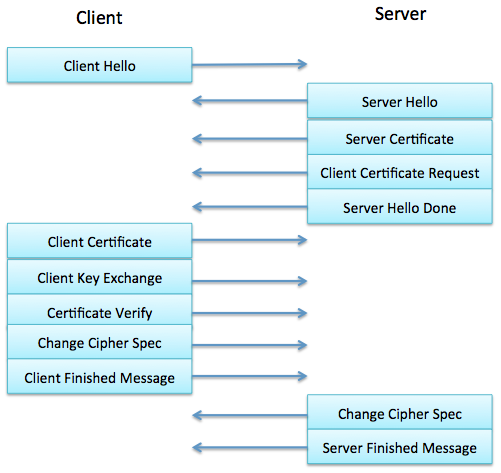
\includegraphics[width=0.7\textwidth]{ssl_handshake.png}
        \label{fig:handshake}
\end{figure}